\section{Análise de imagem}

Analise de imagem é o primeiro passo na analise de dados de nosso sistema, 
no caso desse trabalho a analise deve ter a capacidade de localizar a posição correta das estrelas presentes no campo de visão da câmera.
Erros nesta atapa da analise pode fazer o reconhecimento da posição angular do satélite se tornar impossível.

\subsection{Distorções em imagens}

As correções de distorções nas imagens captadas devem ser realizadas. 
Estas distorções se dividem em dois componentes, uma sendo a radial e outra tangencial, com a componente radial sendo predominante.
Além disto, existem distorções de construção das lentes, distorções de desalinhamento da lente em relação ao centro da Matriz CCD da câmera.

\subsubsection{Distorção radial}
\label{subsubsec:distorcao_radial}

Distorção radial é vista quando utiza-se câmera com grandes ângulos e com pequena distância focal~\cite[]{Mallon}.
Os efeitos da distorção radial são representados na Figura ~\ref{fig:Distorcao_radial}.

\begin{figure}[H]
	\centering
	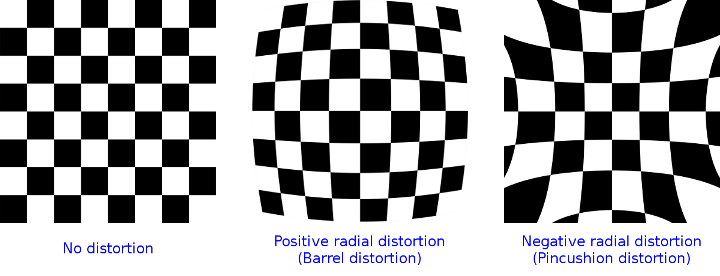
\includegraphics[width=.7\columnwidth]{images/Distorcao_radial.png}
	\caption{Distorção radial. Fonte: ~\cite[]{ozcakir_2020}}
	\label{fig:Distorcao_radial}
\end{figure}

Esta distorção pode ser corrigida através de diferentes métodos, neste trabalho utiliza-se o método matemático descrito pelo ~\cite[]{opencv_library}.
Dessa forma a distorção radial é corrigida através das equações ~\ref{eq:Distorcao_radial_x} e ~\ref{eq:Distorcao_radial_y}.

\begin{equation}
	X_{corrigido} = X_{original} (1 + k_1 r^2 + k_2 r^4 + k_3 r^6),
	\label{eq:Distorcao_radial_x}
\end{equation}

\begin{equation}
	Y_{corrigido} = Y_{original} (1 + k_1 r^2 + k_2 r^4 + k_3 r^6).
	\label{eq:Distorcao_radial_y}
\end{equation}

As equações \ref{eq:Distorcao_radial_x} e \ref{eq:Distorcao_radial_y} são aplicadas para cada pixel da imagem, 
sendo que o valor de $r$ é a distancia em pixels do centro da imagem até o pixel em questão.
O formato destas equações é polinomial, pois quanto maior o valor de $r$ maior a distorção radial.
Para se medir o erro é utilizado uma imagem de referência, com medidas conhecidas, como é visto na Figura ~\ref{fig:Distorcao_radial}.
Em que se utiliza um tabuleiro de xadrez retor para se medir a distorção radial.
Tal efeito polinomial do erro pode ser observado na seção \ref{sec:Resultados_correcao_camera}.

Com o valor de $k_1$, $k_2$ e $k_3$ sendo os coeficientes da correção radial, 
Y original e X original são os valores de pixel da imagem medidos originalmente na imagem,
Y corrigido e X corrigido são os valores de pixel da imagem medidos após a correção radial, 
sendo os valores que a câmera deveria obter se não houvesse distorção radial. 

\subsubsection{Distorção tangencial}
Distorções tangenciais ocorrem quando a câmera e o plano da imagem não estão em paralelo ~\cite[]{ozcakir_2020}.
Os efeitos da distorção tangencial são representados na Figura ~\ref{fig:Distorcao_tangencial}.

\begin{figure}[H]
	\centering
	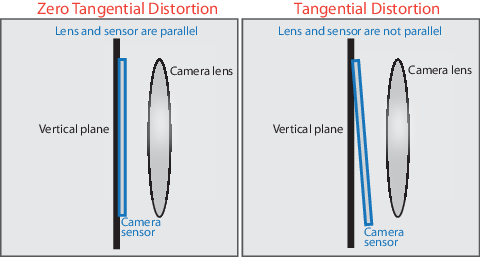
\includegraphics[width=.7\columnwidth]{images/Distorcao_tangencial.png}
	\caption{Distorção tangencial. Fonte: ~\cite[]{ozcakir_2020}}
	\label{fig:Distorcao_tangencial}
\end{figure}

Esta distorção é corrigida através das equações ~\ref{eq:Distorcao_tangencial_x} e ~\ref{eq:Distorcao_tangencial_y}.

\begin{equation}
	X_{corrigido} = X_{original} (1 + p_1 r^2 + p_2 r^4 + p_3 r^6),
	\label{eq:Distorcao_tangencial_x}
\end{equation}

\begin{equation}
	Y_{corrigido} = Y_{original} (1 + p_1 r^2 + p_2 r^4 + p_3 r^6).
	\label{eq:Distorcao_tangencial_y}
\end{equation}

Nas equações \ref{eq:Distorcao_tangencial_x} e \ref{eq:Distorcao_tangencial_y} $r$ é a distância em pixels do centro da imagem até o pixel em questão, 
$p_1$, $p_2$ e $p_3$ são os coeficientes da correção tangencial.
Y

Resalta-se que a ferramenta de simulação estrelar desenvolvida para este trabalho não possui distorcão tangencial, pois a câmera e o plano da imagem estão paralelos.
